%!TEX root=../main.tex
\section{On the geometry of multivariate functional data} % (fold)
\label{sec:geometric_point_of_view_mfpca}

\subsection{Duality diagram} % (fold)
\label{sub:duality_diagram}

The distinction between the space of rows of a matrix as a sample from a population and the space of columns as the fixed variables on which the observations were measured has been explained in \cite{holmesMultivariateDataAnalysis2008} and \cite{delacruzDualityDiagramData2011} for multivariate data analysis. We propose to define a duality diagram in the context of multivariate functional data. Consider the data matrix defined by the set $\mathcal{X}$. \add{We define an operator $L_X : \HH \rightarrow \RR^N$ by
\begin{equation}
    L_X: f \mapsto \begin{pmatrix}
        \sqrt{\pi_1}\inH{X_1 - \mu}{f} \\
        \vdots \\
        \sqrt{\pi_N}\inH{X_N - \mu}{f}
    \end{pmatrix}.
\end{equation}
Using the linearity of the inner-product $\inH{\cdot}{\cdot}$ and vectors, the operator $L_X$ is linear. Define the operator $L^\star_X : \RR^N \rightarrow \HH$ as
\begin{equation}
    L^\star_X: u \mapsto \begin{pmatrix}
       \sum_{n = 1}^N \sqrt{\pi_n} u_n \{X_n^{(1)}(t_1) - \mup{1}(t_1)\} \\ 
       \vdots \\ 
       \sum_{n = 1}^N \sqrt{\pi_n} u_n \{X_n^{(P)}(t_P) - \mup{P}(t_P)\}
    \end{pmatrix}.
\end{equation}
Then $L^\star_X$ is the adjoint operator of the linear operator $L_X$ (see Appendix~\ref{sec:derivation_of_the_inertia_of_the_clouds} for a proof). As an adjoint operator, $L^\star_X$ is a linear operator. The operator $\Gamma$ and the matrix $\mathbf{M}$ define geometries in $\HH$ and $\RR^N$, respectively, through
\begin{equation}
\inHG{f}{g} = \inH{f}{\Gamma g},\quad f, g \in \HH, \quad\text{and}\quad \inRM{u}{v} = u^\top \mathbf{M} v,\quad u, v \in \RR^N.
\end{equation}
We denote by $\normHG{\cdot}$ and $\normRM{\cdot}$ their associated norms.
Using the definition of adjoint operators $L_X$ and $L^\star_X$, we have that
\begin{equation}
    \inRM{L_X(f)}{u} = \inHG{f}{L^\star_X(u)}, \quad\text{for all}\quad f \in \HH, u \in \RR^N.
\end{equation}
These relationships can be expressed as a duality diagram, see Figure~\ref{fig:duality_diagram}. The triplet $(X, \Gamma, \mathbf{M})$ defines a (multivariate) functional data analysis framework. One consequence of this transition between these spaces is that the eigencomponents of $\mathcal{X}$ can indifferently be estimated using the covariance operator $\Gamma$ or the Gram matrix $\mathbf{M}$.} The relationship between the eigecomponents of $\Gamma$ and the eigencomponents of $\mathbf{M}$ are derived in Section~\ref{sec:functional_principal_components_analysis}.
\begin{figure}
    \centering
    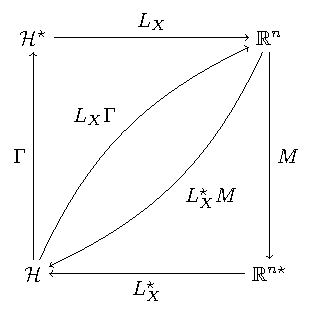
\includegraphics[scale=1.2]{figures/duality_diagram.pdf}
    \caption{Duality diagram between the spaces $\mathcal{H}$ and $\mathbb{R}^N$. The operator $L_X$ and its adjoint $L^\star_X$ are linear operators. The covariance operator $\Gamma$ and the matrix $\mathbf{M}$ define geometries in $\mathcal{H}$ and $\mathbb{R}^N$ respectively. The space $\HH^\star$ (resp. $\RR^{N \star}$) is the dual space of $\HH$ (resp. $\RR^N$).}
    \label{fig:duality_diagram}
\end{figure}

\begin{remark}
   \add{In a general manner, in order to a avoid confusion, inner-products and norms in function space ($\HH$ or $\sLp{\TT{}}$) will be refered with angle brackets, $\inLp{\cdot}{\cdot}$, while inner-products and norms in coordinate space ($\RR^N$) will be refered with round brackets, $\inR{\cdot}{\cdot}$}.
\end{remark}

\begin{remark}\label{rem:rhks}
\add{We present here the duality diagram for the linear integral operator $\Gamma$ with kernel $C$. It is however possible to define duality diagrams for more general linear integral operators defined with continuous symmetric positive definite function as kernel (see \cite{gonzalezRepresentingFunctionalData2010} and \cite{wongNonparametricOperatorregularizedCovariance2019a} for discussions on possible integral operators to represent univariate functional data).}
\end{remark}
% subsection duality_diagram (end)

\subsection{Cloud of individuals} % (fold)
\label{sub:cloud_of_individuals}

\add{Given an element $f \in \HH$, let $\{f^{(p)}(t_p),\,t_p \in \TT{p},\,p = 1, \dots, P\}$ be the features set of the element. We identify this set as the point $\pobs{M}_f$ in the space $\HH$. The space $\HH$ is referred to as the observations' space. The cloud of points that represents the set of observations $\mathcal{X}$ in $\HH$ is denoted by $\CP$. Let $\Gmu$ be the centre of gravity of the cloud $\CP$. In the space $\HH$, its coordinates are given by $\{\mup{p}(t_p),\,t_p \in \TT{p},\,p = 1, \dots, P\}$. If the features are centered, the origin $\OH$ of the axes in $\HH$ coincides with $\Gmu$.}

\begin{figure}
    \centering
    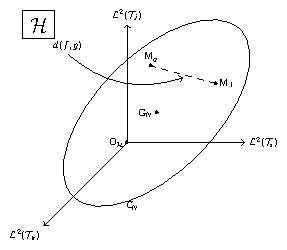
\includegraphics[scale=1.2]{figures/cloud_obs.pdf}
    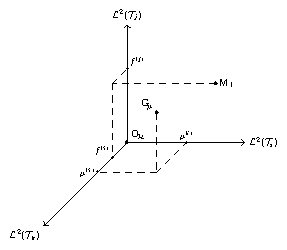
\includegraphics[scale=1.2]{figures/cloud_obs_proj.pdf}
    \caption{Left: Cloud of observations. Right: Projection of the points onto the elements of $\HH$. The observation $f$ (resp. $g$) is identified by the point $\pobs{M}_f$ (resp. $\pobs{M}_g$) in the cloud $\CP$. The point $\Gmu$ is the center of gravity of $\CP$ and the point $\OH$ is the origin of the space $\HH$.}
    \label{fig:cloud_obs}
\end{figure}

\add{Let $f$ and $g$ be two elements in $\HH$ and denote by $\pobs{M}_f$ and $\pobs{M}_g$ their associated points in $\CP$ (see Figure~\ref{fig:cloud_obs}). The most natural distance between these observations is based on the usual inner product in $\HH$, $\inH{\cdot}{\cdot}$, and is defined as
\begin{equation}\label{eq:distance_obs}
    d^2(\pobs{M}_f, \pobs{M}_g) = \normH{f - g}^2 = \sum_{p = 1}^P \int_{\TT{p}}\left\{\fp(t_p) - \gp(t_p)\right\}^2 \dd t_p.
\end{equation}
This distance measures how different the observations are, and thus gives one characterization of the shape of the cloud $\CP$. Another description of this shape is to consider the distance between each observation and $\Gmu$, the center of the cloud. Let $f$ be an element of $\HH$, associated to the point $\pobs{M}_f$, and $\mu$ the element of $\HH$ related to $\Gmu$, the distance between $f$ and $\mu$ is given by
\begin{equation}\label{eq:distance_center}
    d^2(\pobs{M}_f, \Gmu) = \normH{f - \mu}^2 = \sum_{p = 1}^P \int_{\TT{p}}\left\{\fp(t_p) - \mup{p}(t_p)\right\}^2 \dd t_p.
\end{equation}
Given the set $\XX$, the total inertia of $\CP$, with respect to $\Gmu$ and the distance $d$, is given by
\begin{equation}\label{eq:inertia}
    \sum_{n = 1}^N \pi_n d^2(\pobs{M}_n, \Gmu) = \frac{1}{2}\sum_{i = 1}^N \sum_{j = 1}^N \pi_i \pi_j d^2(\pobs{M}_i, \pobs{M}_j) = \sum_{p = 1}^P \int_{\TT{p}}\Var{\Xp{p}(t_p)} \dd t_p.
\end{equation}}
\add{The duality diagram, however, allows us to defined another suitable distance to characterize the shape of the cloud $\CP$. We thus define
\begin{equation}
    d^2_\Gamma(\pobs{M}_f, \pobs{M}_g) = \normHG{f - g}^2.
\end{equation}
The utilization of the distance measure $d_\Gamma$, which accounts for the variability among all the features within the functional data, corresponds to a Mahalanobis-type distance framework for multivariate functional data (see \cite{berrenderoMahalanobisDistanceFunctional2020} and \cite{martinoKmeansProcedureBased2019}).
Given the set $\XX$, the total inertia of $\CP$, with respect to $\Gmu$ and the distance $d_\Gamma$, is given by
\begin{equation}\label{eq:inertia_CP}
    \sum_{n = 1}^N \pi_n d_\Gamma^2(\pobs{M}_n, \Gmu) = \frac{1}{2}\sum_{i = 1}^N \sum_{j = 1}^N \pi_i \pi_j d_\Gamma^2(\pobs{M}_i, \pobs{M}_j) = \sum_{p = 1}^P \int_{\TT{p}} \normH{C_{p \cdot}(t_p, \cdot)}^2 \dd t_p.
\end{equation}
The derivation of these equalities are given in Appendix \ref{sec:derivation_of_the_inertia_of_the_clouds}.}

\begin{remark}
    These results have the same interpretation as for multivariate scalar data. This is also the multivariate analogue of the relation between variance and sum of squared differences known for univariate functional data. \add{If the features are reduced beforehand, such that $\int_{\TT{p}} \Var\Xp{p} (t_p) \dd t_p = 1$ for the distance $d$ or $\int_{\TT{p}} \normH{C_{p \cdot}(t_p, \cdot)}^2 \dd t_p = 1$ for the distance $d_\Gamma$, the total inertia of the cloud $\CP$ is equal to the number of components $P$. We are, in general, not interested by the total inertia but mostly how this variance is spread among the features.}
\end{remark}

% subsection cloud_of_individuals (end)

\subsection{Cloud of features} % (fold)
\label{sub:cloud_of_features}

\add{Given an element $f \in \HH$, let $L_X(f) = \{\sqrt{\pi_n}\inH{X_n - \mu}{f},\,n = 1, \dots, N\}$ be the set of projections of $f$ onto the centered observations. We identify this set as the point $\pfea{M}_f$ in the space $\RR^N$. The space $\RR^N$ is referred to as the features' space. The cloud of points that represents the set of observations in $\RR^N$ is denoted by $\CN$. Let $\Gfea$ be the centre of gravity of the cloud $\CN$. In the space $\RR^N$, its coordinates are given by $L_X(\mu) = \{\sqrt{\mu}\inH{X_n - \mu}{\mu},\,n = 1, \dots, N\}$. If the data are centered, the origin $\OG$ of the axes in $\RR^N$ coincides with $\Gfea$.}

\begin{figure}
    \centering
    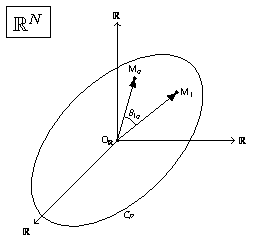
\includegraphics[scale=1.2]{figures/cloud_features.pdf}
    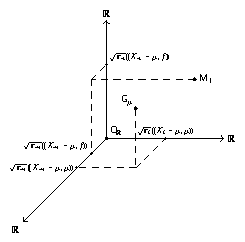
\includegraphics[scale=1.2]{figures/cloud_features_proj.pdf}
    \caption{Left: Cloud of features. Right: Projection of the points on the elements of $\RR^N$. The observation $f$ (resp. $g$) is identified by the point $\pfea{M}_f$ (resp. $\pfea{M}_g$) in the cloud $\CN$. The point $\Gfea$ is the center of gravity of $\CN$ and the point $\OG$ is the origin of the space $\RR^N$.}
    \label{fig:cloud_features}
\end{figure}

\add{We consider the usual inner-product in $\RR^N$, such that for all $u, v \in \RR^N, \inR{u}{v} = u^\top v$, associated with the norm $\normR{\cdot}$. Let $f$ and $g$ be two elements in $\HH$ and denote by $\pfea{M}_f$ and $\pfea{M}_g$ their associated points in $\CN$ (see Figure~\ref{fig:cloud_features}). The distance between $\pfea{M}_f$ and $\pfea{M}_g$ is thus defined as
\begin{equation*}
\mathsf{d}^2(\pfea{M}_f, \pfea{M}_g) = \normR{L_X(f) - L_X(g)}^2 = \sum_{n = 1}^N \pi_n \inH{X_n - \mu}{f - g}^2.
\end{equation*}}
\add{Similarly to the cloud of individuals, this distance characterize the shape of the cloud $\CN$ and we also have access to this characterization through the distance with the center of gravity $\Gfea$. Let $f$ be an element of $\HH$, associated to the point $\pfea{M}_f$, and $\mu$ the element of $\HH$ related to $\Gfea$, the distance between $\pfea{M}_f$ and $\mu$ is given by
\begin{equation*}
\mathsf{d}^2(\pfea{M}_f, \Gfea) = \normR{L_X(f) - L_X(\mu)}^2 = \sum_{n = 1}^N \pi_n \inH{X_n - \mu}{f - \mu}^2.
\end{equation*}
Given the set $\XX$, the total inertia of $\CN$, with respect to $\Gfea$ and the distance $\mathsf{d}$, is given by
\begin{equation}\label{eq:inertia_CN}
    \sum_{n = 1}^N \pi_n \mathsf{d}^2(\pfea{M}_n, \Gfea) = \frac{1}{2}\sum_{i = 1}^N \sum_{j = 1}^N \pi_i \pi_j \mathsf{d}^2(\pfea{M}_i, \pfea{M}_j) = \sum_{p = 1}^P \int_{\TT{p}} \normH{C_{p \cdot}(t_p, \cdot)}^2 \dd t_p.
\end{equation}
Using the distances induced by the duality diagram, the total inertia of the cloud $\CN$ is thus equal to the total inertia of the cloud $\CP$. This property highlights the duality between the spaces $\HH$ and $\RR^N$. To further emphasize this duality, the cosine of the angle $\theta_{fg}$ formed by the two points $\pfea{M}_f$ and $\pfea{M}_g$ is equal to their correlation coefficient and can be written
\begin{equation}
    \cos(\theta_{fg}) = \frac{\inR{L_X(f)}{L_X(g)}}{\normR{L_X(f)}\normR{L_X(g)}}
    = \frac{\inHG{f}{g}}{\normHG{f}\normHG{g}}.
\end{equation}}
The derivation of these equalities are given in Appendix \ref{sec:derivation_of_the_inertia_of_the_clouds}.

\begin{remark}
   Although each axis of the space does not directly represent the features, but rather the projection of an element of $\HH$ onto the elements of the set $\XX$, we refer to this space as the features' space. We use this terminology to highlight the similarity between multivariate functional data analysis and traditional multivariate data analysis, as well as to emphasize the dimensionality of this space.
\end{remark}
% subsection cloud_of_features (end)

\subsection{On centering and reducing} % (fold)
\label{sub:on_centering_and_reducing}

For conducting an MFPCA, the features are usually assumed centred \citep{happMultivariateFunctionalPrincipal2018a}. \cite{protheroNewPerspectivesCentering2023} give a complete overview of centering in the context of FDA. Here, we comment on the geometric interpretation of centering in this context and compare with the multivariate scalar case. We focus on the usual centering in FDA, namely $\Xnp(t_p) - \mu^{(p)}(t_p),~t_p \in \TT{p}$ (refered as \emph{object centering} in \cite{protheroNewPerspectivesCentering2023}).
\add{The geometric interpretation of the object centering is the same if we refer to the observations' space $\HH$ or the features' space $\RR^N$. Within the space $\HH$ (resp. $\RR^N$), centering is interpreted as translating the centre of gravity of the clouds, $\Gmu$ (resp. $\Gfea$), to the origin point $\OH$ (resp. $\OG$) of the space $\HH$ (resp. $\RR^N$). This transformation, being a translation, does not change the shape of the cloud $\CP$ (resp. $\CN$). The interpretation is the same as for the centering in the multivariate scalar data context within their observation space.}

Concerning the standardization of the data, there are two main proposals in the literature. \cite{happMultivariateFunctionalPrincipal2018a} propose to weight each component $p$ by
\begin{equation}
w_p = \left(\int_{\TT{p}} \Var X^{(p)}(t_p) \dd t_p\right)^{-1}.
\end{equation}
This standardization is coherent with the derivation of the total inertia of the observations' space using the usual distance in $\HH$. \cite{chiouMultivariateFunctionalPrincipal2014} propose to standardize each component $p$ of the data using the function
\begin{equation}
w_p(t_p) = \left(\Var X^{(p)}(t_p)\right)^{-1/2}, \quad t_p \in \TT{p}.
\end{equation}
This corresponds to a standardization of the curves by the standard deviation of the component at each sampling point. The standard deviation curve is estimated as the square root of the diagonal of the covariance function estimates, obtained using a local linear smoother of the pooled data. \add{For each functional feature $p$, this standardization mimics the standardization used for principal components analysis if the number of (scalar) features is infinite.}
\add{Considering the duality diagram and the total inertia of the clouds with respect to the distance $d_\Gamma$, we propose to weight each component $p$ by
\begin{equation}
    w_p = \left(\int_{\TT{p}} \normH{C_{p \cdot}(t_p, \cdot)}^2 \dd t_p\right)^{-1/2}.
\end{equation}
The total inertia of $\CP$ (and $\CN$) will thus be equal to the number of components.}

% subsection on_centering_and_reducing (end)

% section sec:geometric_point_of_view_mfpca (end)